\documentclass[border=6pt]{standalone}
\usepackage{tikz}
\usetikzlibrary{arrows.meta,positioning,calc,fit,backgrounds}

\definecolor{ink}{HTML}{0F172A}
\definecolor{muted}{HTML}{64748B}
\definecolor{linegray}{HTML}{CBD5E1}
\definecolor{panel}{HTML}{F8FAFC}
\definecolor{gearfill}{HTML}{EEF2FF}
\definecolor{gearstroke}{HTML}{4F46E5}
\definecolor{fusefill}{HTML}{FEF2F2}
\definecolor{fusestroke}{HTML}{DC2626}
\definecolor{loadfill}{HTML}{FFF7ED}
\definecolor{loadstroke}{HTML}{EA580C}
\definecolor{wire24}{HTML}{2563EB}
\definecolor{wire12}{HTML}{7C3AED}
\definecolor{wire48}{HTML}{B91C1C}

\begin{document}
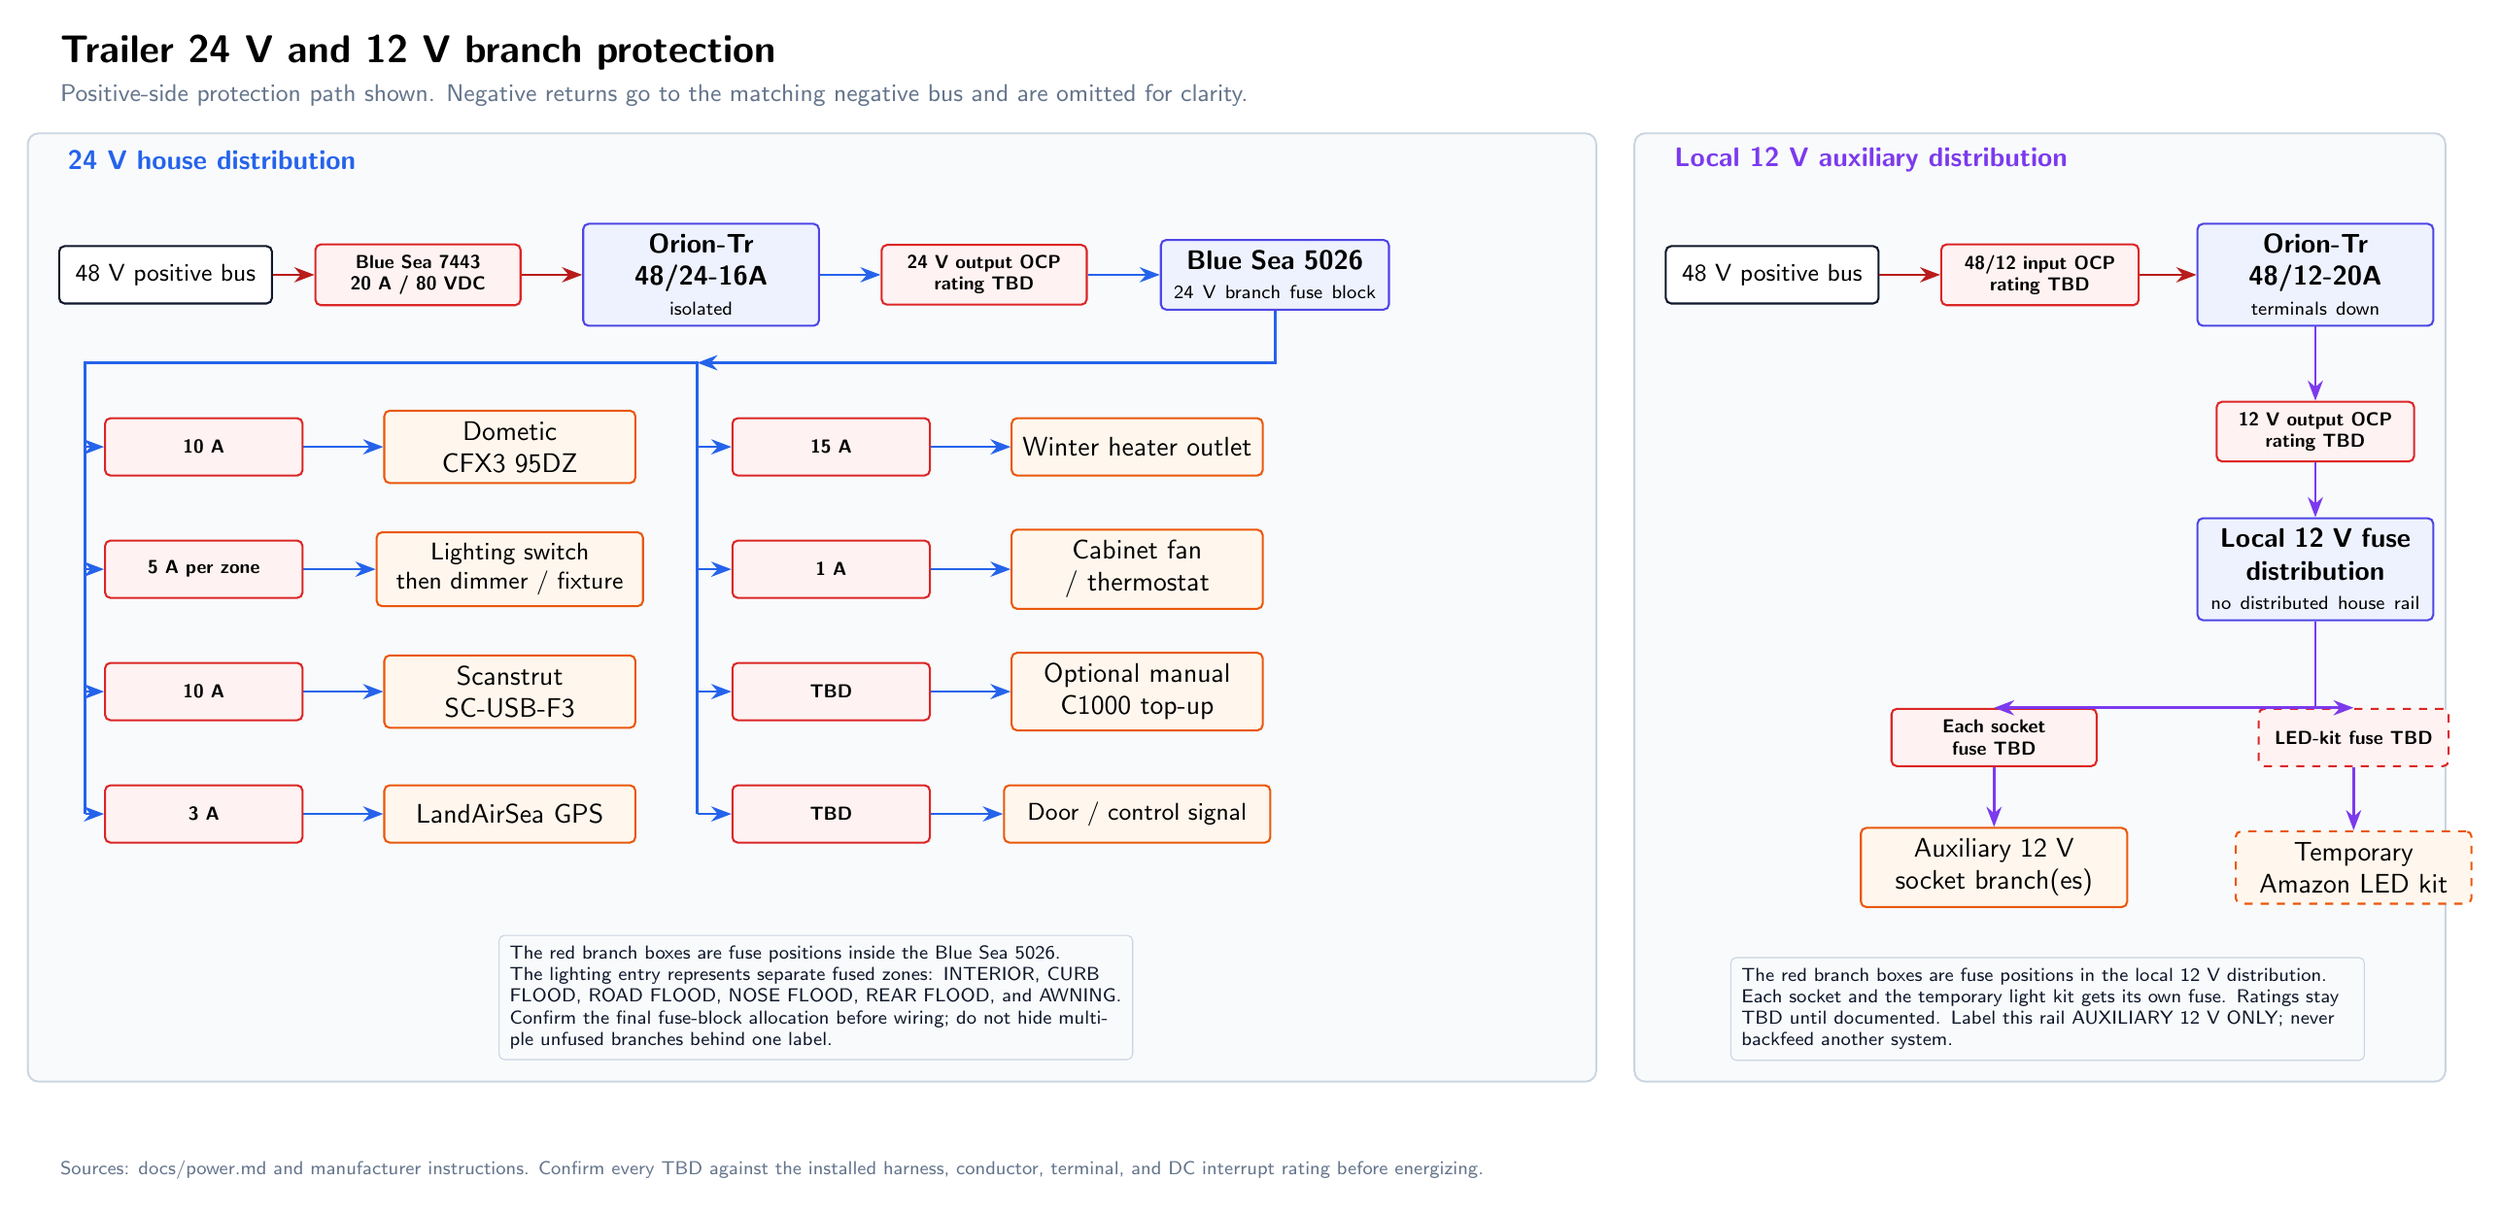
\begin{tikzpicture}[
  font=\sffamily,
  >=Stealth,
  block/.style={draw=ink, fill=white, rounded corners=2pt, line width=0.75pt,
    align=center, inner sep=4pt, minimum height=0.75cm},
  gear/.style={block, fill=gearfill, draw=gearstroke},
  fuse/.style={block, fill=fusefill, draw=fusestroke, font=\sffamily\scriptsize\bfseries},
  load/.style={block, fill=loadfill, draw=loadstroke},
  note/.style={draw=linegray, fill=panel, rounded corners=2pt, align=left,
    inner sep=4pt, font=\sffamily\scriptsize, text=ink},
  zone/.style={draw=linegray, fill=panel, rounded corners=4pt, line width=0.7pt},
  wfortyeight/.style={->, draw=wire48, line width=1.0pt},
  wtwentyfour/.style={->, draw=wire24, line width=1.0pt},
  wtwelve/.style={->, draw=wire12, line width=1.0pt}
]

\node[font=\sffamily\bfseries\Large, anchor=west] at (0,14.6)
  {Trailer 24 V and 12 V branch protection};
\node[font=\sffamily\small, text=muted, anchor=west] at (0,14.05)
  {Positive-side protection path shown. Negative returns go to the matching negative bus and are omitted for clarity.};

\begin{scope}[on background layer]
  \node[zone, fit={(-0.3,1.15) (20.2,13.55)}, inner sep=0pt] {};
  \node[zone, fit={(20.7,1.15) (31.3,13.55)}, inner sep=0pt] {};
\end{scope}

\node[font=\sffamily\bfseries, anchor=west, text=wire24] at (0.1,13.2) {24 V house distribution};
\node[block, text width=2.5cm, font=\sffamily\small] (bus48a) at (1.5,11.7) {48 V positive bus};
\node[fuse, text width=2.4cm] (in24) at (4.8,11.7) {Blue Sea 7443\\20 A / 80 VDC};
\node[gear, text width=2.8cm] (orion24) at (8.5,11.7)
  {\textbf{Orion-Tr 48/24-16A}\\[-1pt]\scriptsize isolated};
\node[fuse, text width=2.4cm] (out24) at (12.2,11.7)
  {24 V output OCP\\rating TBD};
\node[gear, text width=2.7cm] (fuseblock) at (16.0,11.7)
  {\textbf{Blue Sea 5026}\\[-1pt]\scriptsize 24 V branch fuse block};
\draw[wfortyeight] (bus48a) -- (in24);
\draw[wfortyeight] (in24) -- (orion24);
\draw[wtwentyfour] (orion24) -- (out24);
\draw[wtwentyfour] (out24) -- (fuseblock);

\node[fuse, text width=2.3cm] (fridgef) at (2.0,9.45) {10 A};
\node[load, text width=3.0cm] (fridge) at (6.0,9.45) {Dometic CFX3 95DZ};
\node[fuse, text width=2.3cm] (lightf) at (2.0,7.85) {5 A per zone};
\node[load, text width=3.2cm, font=\sffamily\small] (lights) at (6.0,7.85) {Lighting switch\\then dimmer / fixture};
\node[fuse, text width=2.3cm] (usbf) at (2.0,6.25) {10 A};
\node[load, text width=3.0cm] (usb) at (6.0,6.25) {Scanstrut SC-USB-F3};
\node[fuse, text width=2.3cm] (gpsf) at (2.0,4.65) {3 A};
\node[load, text width=3.0cm] (gps) at (6.0,4.65) {LandAirSea GPS};
\node[fuse, text width=2.3cm] (heaterf) at (10.2,9.45) {15 A};
\node[load, text width=3.0cm] (heater) at (14.2,9.45) {Winter heater outlet};
\node[fuse, text width=2.3cm] (fanf) at (10.2,7.85) {1 A};
\node[load, text width=3.0cm] (fan) at (14.2,7.85) {Cabinet fan / thermostat};
\node[fuse, text width=2.3cm] (topupf) at (10.2,6.25) {TBD};
\node[load, text width=3.0cm] (topup) at (14.2,6.25) {Optional manual C1000 top-up};
\node[fuse, text width=2.3cm] (signalf) at (10.2,4.65) {TBD};
\node[load, text width=3.2cm, font=\sffamily\small] (signal) at (14.2,4.65) {Door / control signal};

\coordinate (left24trunk) at (0.45,9.45);
\coordinate (right24trunk) at (8.45,9.45);
\draw[draw=wire24, line width=1.0pt] (0.45,4.65) -- (0.45,10.55)
  -- (8.45,10.55) -- (8.45,4.65);
\draw[wtwentyfour] (fuseblock.south) |- (8.45,10.55);

\foreach \f/\l in {fridgef/fridge,lightf/lights,usbf/usb,gpsf/gps}{
  \draw[wtwentyfour] (left24trunk |- \f.west) -- (\f.west);
  \draw[wtwentyfour] (\f.east) -- (\l.west);
}
\foreach \f/\l in {heaterf/heater,fanf/fan,topupf/topup,signalf/signal}{
  \draw[wtwentyfour] (right24trunk |- \f.west) -- (\f.west);
  \draw[wtwentyfour] (\f.east) -- (\l.west);
}

\node[note, text width=8.0cm] at (10.0,2.25)
  {The red branch boxes are fuse positions inside the Blue Sea 5026. The lighting entry represents separate fused zones: INTERIOR, CURB FLOOD, ROAD FLOOD, NOSE FLOOD, REAR FLOOD, and AWNING. Confirm the final fuse-block allocation before wiring; do not hide multiple unfused branches behind one label.};

\node[font=\sffamily\bfseries, anchor=west, text=wire12] at (21.1,13.2) {Local 12 V auxiliary distribution};
\node[block, text width=2.5cm, font=\sffamily\small] (bus48b) at (22.5,11.7) {48 V positive bus};
\node[fuse, text width=2.3cm] (in12) at (26.0,11.7) {48/12 input OCP\\rating TBD};
\node[gear, text width=2.8cm] (orion12) at (29.6,11.7)
  {\textbf{Orion-Tr 48/12-20A}\\[-1pt]\scriptsize terminals down};
\draw[wfortyeight] (bus48b) -- (in12);
\draw[wfortyeight] (in12) -- (orion12);

\node[fuse, text width=2.3cm] (out12) at (29.6,9.65) {12 V output OCP\\rating TBD};
\node[gear, text width=2.8cm] (fuse12) at (29.6,7.85)
  {\textbf{Local 12 V fuse distribution}\\[-1pt]\scriptsize no distributed house rail};
\draw[wtwelve] (orion12) -- (out12);
\draw[wtwelve] (out12) -- (fuse12);

\node[fuse, text width=2.4cm] (socketf) at (25.4,5.65) {Each socket fuse TBD};
\node[load, text width=3.2cm] (sockets) at (25.4,3.95) {Auxiliary 12 V socket branch(es)};
\node[fuse, dashed, text width=2.2cm] (ledf) at (30.1,5.65) {LED-kit fuse TBD};
\node[load, dashed, text width=2.8cm] (led) at (30.1,3.95) {Temporary Amazon LED kit};
\draw[wtwelve] (fuse12.south) |- (socketf.north);
\draw[wtwelve] (socketf) -- (sockets);
\draw[wtwelve] (fuse12.south) |- (ledf.north);
\draw[wtwelve] (ledf) -- (led);

\node[note, text width=8.0cm] at (26.1,2.1)
  {The red branch boxes are fuse positions in the local 12 V distribution. Each socket and the temporary light kit gets its own fuse. Ratings stay TBD until documented. Label this rail AUXILIARY 12 V ONLY; never backfeed another system.};

\node[font=\sffamily\scriptsize, text=muted, anchor=west] at (0,0)
  {Sources: docs/power.md and manufacturer instructions. Confirm every TBD against the installed harness, conductor, terminal, and DC interrupt rating before energizing.};
\end{tikzpicture}
\end{document}
